\documentclass[letterpaper,journal]{IEEEtran}

\usepackage{amsmath,amsfonts}
\usepackage{array}
\usepackage{booktabs}
\usepackage{cite}
\usepackage{graphicx}
\usepackage{siunitx}
\usepackage{url}

\graphicspath{{figures_tie/}{../analysis_ready/matlab_B_results/}{../figures/}}
\hyphenation{magneto-enceph-alo-graphy nano-crys-tal-line com-pen-sa-tion}
\sisetup{detect-all}

\begin{document}

\title{Modeling and Application-Oriented Optimization of Hybrid Multilayer Ferrite Magnetic Shields for SERF-MEG Magnetometers}

\author{Author~Name%
\thanks{Author affiliation, funding, and correspondence information should be added before submission.}
}

\markboth{IEEE Transactions on Instrumentation and Measurement}%
{Author: Hybrid Multilayer Ferrite Magnetic Shield}

\maketitle

\begin{abstract}
SERF-based magnetoencephalography requires a magnetic shielding environment with high shielding factor, low residual field, and controlled shield-induced magnetic-noise contribution. This paper formulates a hybrid multilayer magnetic shield in which flexible ferrite sheets form a low-conductivity base and an amorphous or nanocrystalline ribbon provides an additional high-permeability magnetic path. The ferrite base has an inner radius of \SI{100}{mm} and an axial length of \SI{200}{mm}. A four-layer ferrite candidate with \SI{0.15}{mm} sheets and \SI{0.08}{mm} radial gaps is selected as a manufacturable validation base under total-thickness, radial-space, flexibility, assembly, shielding-factor, and IntH2 constraints, not as a global optimum. The finite-element model uses directional no-shield references and component-based shielding factors. In the transverse direction, the ferrite-only base gives $\mathrm{SF}_x=3.629$ and $\mathrm{IntH2}_{\mathrm{total}}=4.160\times10^{-6}$. Adding an amorphous outer layer increases $\mathrm{SF}_x$ to 8.548 and reduces $\mathrm{IntH2}_{\mathrm{total}}$ to $6.283\times10^{-7}$, while adding a nanocrystalline outer layer increases $\mathrm{SF}_x$ to 25.146 and reduces $\mathrm{IntH2}_{\mathrm{total}}$ to $5.333\times10^{-8}$ under the present initial-permeability assumptions. Axial cap simulations show that a single nanocrystalline cap improves $\mathrm{SF}_z$ from 2.412 to 2.907 but introduces an IntH2 tradeoff. Prototype shielding-factor measurement, low-field permeability/loss characterization, compensation-coil nulling, and magnetometer PSD measurement remain required before claiming instrument-level sensitivity improvement.
\end{abstract}

\begin{IEEEkeywords}
Amorphous ribbon, ferrite magnetic shield, finite-element method, flexible magnetic shielding, magnetic noise, nanocrystalline ribbon, SERF-MEG, shielding factor.
\end{IEEEkeywords}

\section{Introduction}
\IEEEPARstart{S}{ERF-based} magnetoencephalography (MEG) and optically pumped magnetometer (OPM) systems require a low-field and low-noise magnetic environment because femtotesla-level biomagnetic signals can be obscured by residual environmental fields and by magnetic noise generated inside the shield itself \cite{ref1,ref2,ref3,ref4}. The magnetic shield is therefore not only a passive attenuation component. It must be evaluated by directional shielding factor, residual center field, and material-loss-related magnetic-noise indicators.

High-permeability metallic shields such as permalloy and mu-metal are widely used to attenuate static and low-frequency magnetic fields \cite{ref6,ref7,ref8}. However, their electrical conductivity and material loss can introduce low-frequency magnetic noise in magnetometer applications \cite{ref9,ref10,ref11}. Ferrites are attractive for low-noise shielding because of their high electrical resistivity and reduced eddy-current loss \cite{ref12,ref13,ref14,ref16}. The limitation is that the shielding factor of a thin and flexible ferrite cylinder can be modest when radial space and total thickness are constrained.

Amorphous and nanocrystalline ribbons are commercially available high-permeability soft-magnetic materials. Compared with rigid metallic shells, ribbon-based amorphous or nanocrystalline layers can be more compatible with low-cost and flexible shield fabrication. This motivates a hybrid structure: ferrite sheets provide a low-conductivity base, while an additional amorphous or nanocrystalline ribbon provides a high-permeability magnetic path. The proposed shield is therefore not a ferrite-only multilayer cylinder, but a composite magnetic shielding structure for compact SERF-MEG instrumentation.

The present manuscript deliberately separates simulated shielding improvement from experimental sensitivity claims. The finite-element model uses representative initial relative permeability values for low-field operation. Since the shield is intended to operate near the geomagnetic field without strong excitation, these values are interpreted as the slope of the $B$--$H$ curve around $H=0$. The amorphous and nanocrystalline permeability and magnetic-loss parameters must be updated after material characterization.

The contributions of this paper are as follows:
\begin{enumerate}
\item A four-layer ferrite base is selected as a manufacturable validation candidate under thickness, radial-space, flexibility, assembly, $\mathrm{SF}$, and IntH2 constraints.
\item Amorphous and nanocrystalline outer layers are compared as hybrid transverse-shielding enhancement candidates.
\item A single-ended axial cap is evaluated as an axial leakage-suppression approach with an explicit $\mathrm{SF}_z$--IntH2 tradeoff.
\item A material-separated noise proxy is introduced to prevent simulation IntH2 from being overinterpreted as measured magnetometer noise.
\item A P0/P1/P2 prototype validation route is defined, including shielding-factor measurement, low-field permeability/loss measurement, compensation-coil nulling, and magnetometer PSD measurement.
\end{enumerate}

\begin{figure*}[!t]
\centering
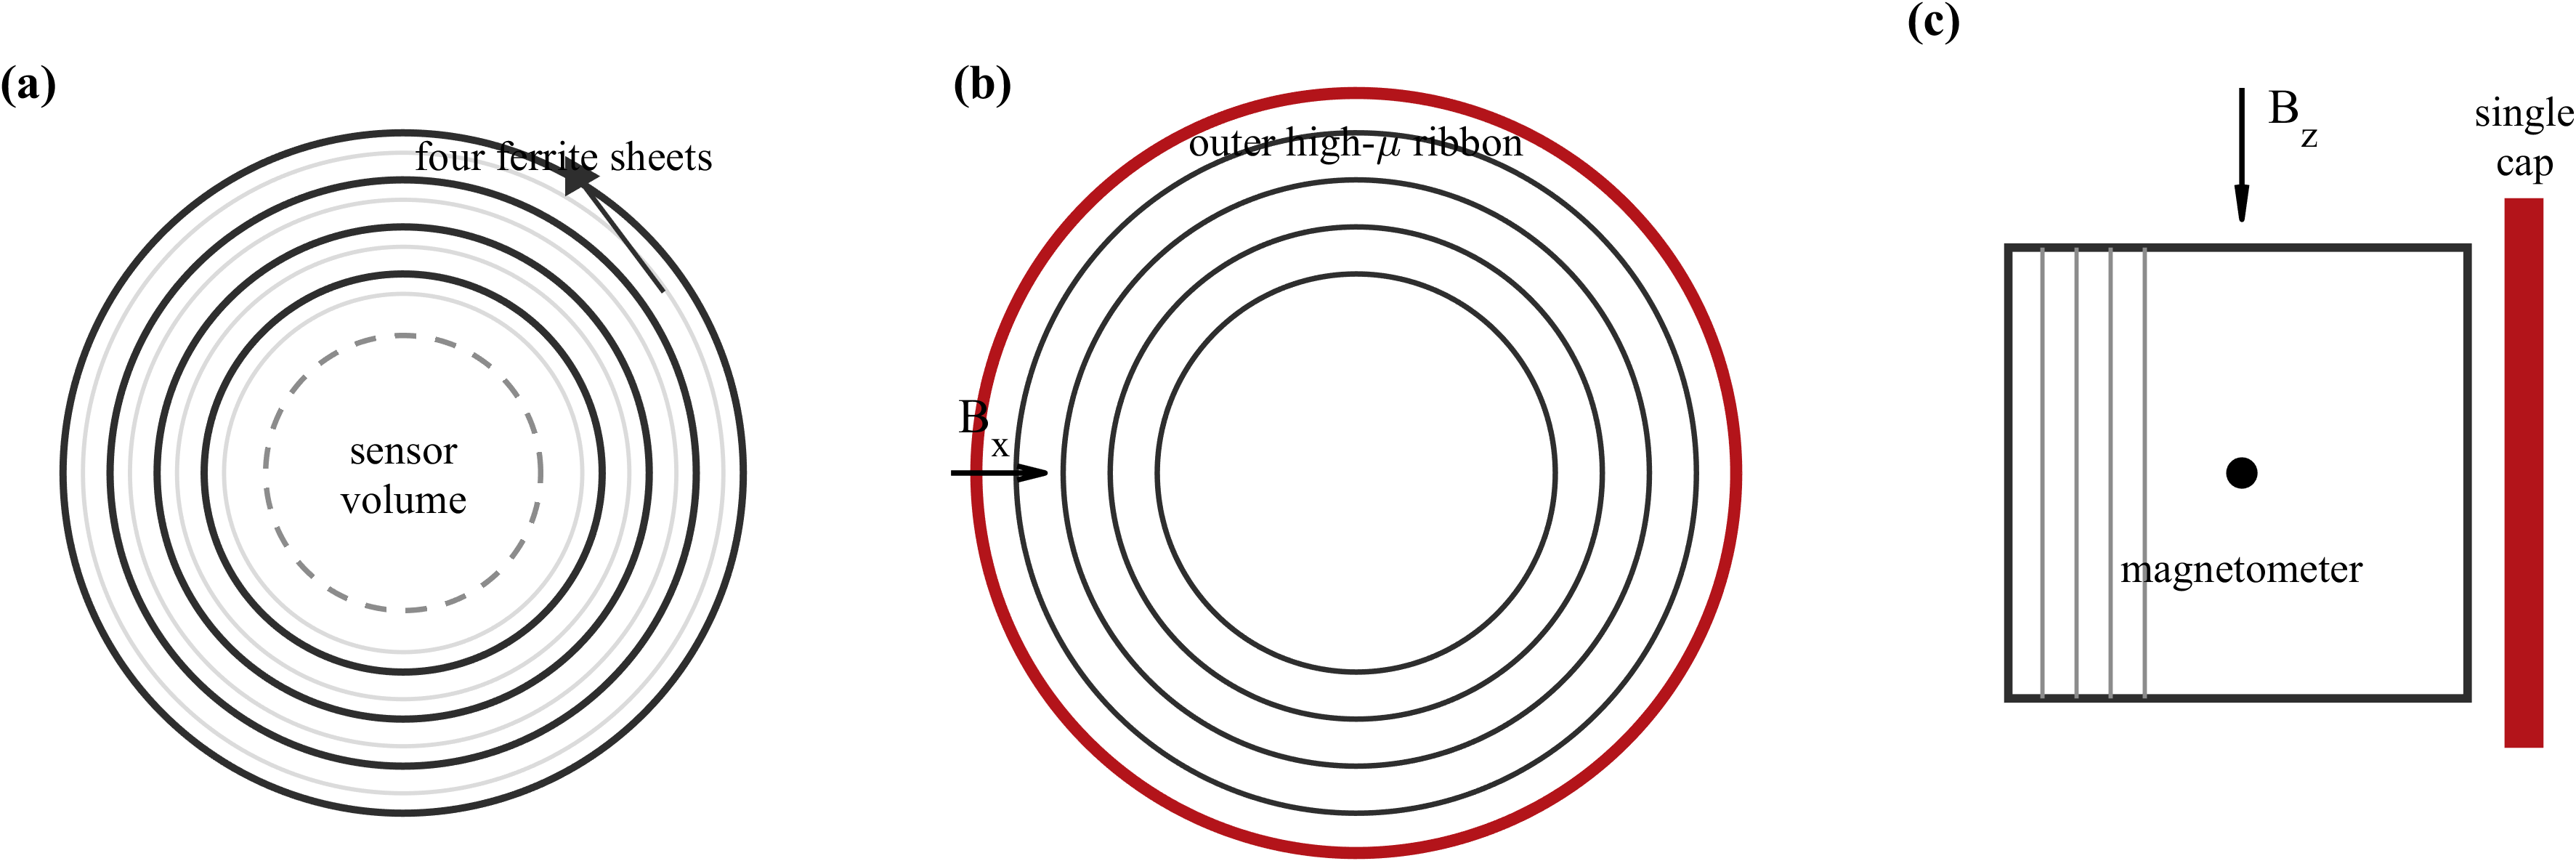
\includegraphics[width=0.92\textwidth]{Fig01_concept_hybrid_multilayer_shield.png}
\caption{Concept of the hybrid multilayer ferrite shield for magnetometer applications. (a) Four-layer ferrite base. (b) Outer amorphous or nanocrystalline high-permeability layer. (c) Single-ended cap and magnetometer placement.}
\label{fig:concept}
\end{figure*}

\section{Principle of Hybrid Multilayer Magnetic Shielding}

\subsection{Shielding Factor and Leakage Ratio}

For an external field applied along $q\in\{x,y,z\}$, the no-shield reference field at the observation point is
\begin{equation}
\mathbf{B}_0=(B_{0,x},B_{0,y},B_{0,z}),
\label{eq:b0}
\end{equation}
and the shielded center leakage field is
\begin{equation}
\mathbf{B}_{\mathrm{center}}=(B_{\mathrm{center},x},B_{\mathrm{center},y},B_{\mathrm{center},z}).
\label{eq:bcenter}
\end{equation}
The directional shielding factor is
\begin{equation}
\mathrm{SF}_q=\frac{|B_{0,q}|}{|B_{\mathrm{center},q}|},
\label{eq:sfq}
\end{equation}
and the leakage ratio is
\begin{equation}
\mathrm{LeakageRatio}_q=\frac{|B_{\mathrm{center},q}|}{|B_{0,q}|}.
\label{eq:leakage}
\end{equation}
The formal shielding factor is computed from the intended field component. The vector magnitude is retained only as an auxiliary consistency check and is not used as the primary $\mathrm{SF}$ definition.

\subsection{Magnetic-Noise-Related IntH2 Metric}

The shield-induced magnetic noise can be related to material loss through the fluctuation-dissipation theorem \cite{ref9,ref18}. A virtual pickup coil placed at the observation point produces a magnetic field $H_{\mathrm{vc}}$ in the magnetic material. The finite-element exported geometry-dependent indicator is
\begin{equation}
\mathrm{IntH2}=\int_V H_{\mathrm{vc}}^2\,dV.
\label{eq:inth2}
\end{equation}
It becomes an absolute magnetic-noise prediction only after measured $\mu''(f)$, temperature, frequency, and virtual-coil normalization are specified.

For hybrid structures, the integration must include both the ferrite layers and the added soft-magnetic ribbon. The material-separated form is
\begin{equation}
\mathrm{IntH2}_{\mathrm{total}}
=
\mathrm{IntH2}_{\mathrm{ferrite}}
+
\mathrm{IntH2}_{\mathrm{metal}} .
\label{eq:inth2sep}
\end{equation}
The corresponding noise proxy is proportional to
\begin{equation}
P_{\mathrm{noise}}
\propto
\mu''_{\mathrm{ferrite}}\mathrm{IntH2}_{\mathrm{ferrite}}
+
\mu''_{\mathrm{metal}}\mathrm{IntH2}_{\mathrm{metal}} .
\label{eq:noiseproxy}
\end{equation}
Thus, a lower $\mathrm{IntH2}_{\mathrm{total}}$ under equal-loss assumptions is favorable, but it is not a proof of lower measured shield noise unless the material loss and magnetometer PSD are measured.

\subsection{Hybrid Outer-Layer and Axial Cap Concepts}

The ferrite base provides a low-conductivity and flexible shield body. The amorphous or nanocrystalline outer layer provides a higher-permeability magnetic path that improves transverse attenuation. In the present stage, amorphous and nanocrystalline ribbons are modeled with representative initial relative permeability values for low-field operation. These values are placeholders for measured low-field $B$--$H$ slopes and magnetic-loss data.

Open-ended cylindrical shields generally leak in the axial direction. A single-ended cap is therefore introduced to reduce axial leakage while preserving a practical opening. A small axial gap between the cylindrical shield and the cap represents mechanical support and avoids an unrealistically sharp zero-gap contact in the FEM mesh.

\section{FEM Model and Structural Design Matrix}

\subsection{Four-Layer Ferrite Base}

The selected ferrite base has inner radius $R_{\mathrm{in}}=\SI{100}{mm}$ and axial length $L=\SI{200}{mm}$. Four ferrite sheets of thickness $t=\SI{0.15}{mm}$ are separated by $g=\SI{0.08}{mm}$ gaps. The total ferrite thickness is \SI{0.60}{mm}, and the radial occupation is \SI{0.84}{mm}. Although increasing the number of ferrite sheets may further improve shielding, the multilayer stack becomes increasingly difficult to bend and assemble. The four-layer ferrite base is therefore selected as a manufacturable validation candidate, not as a global optimum.

\begin{figure}[!t]
\centering
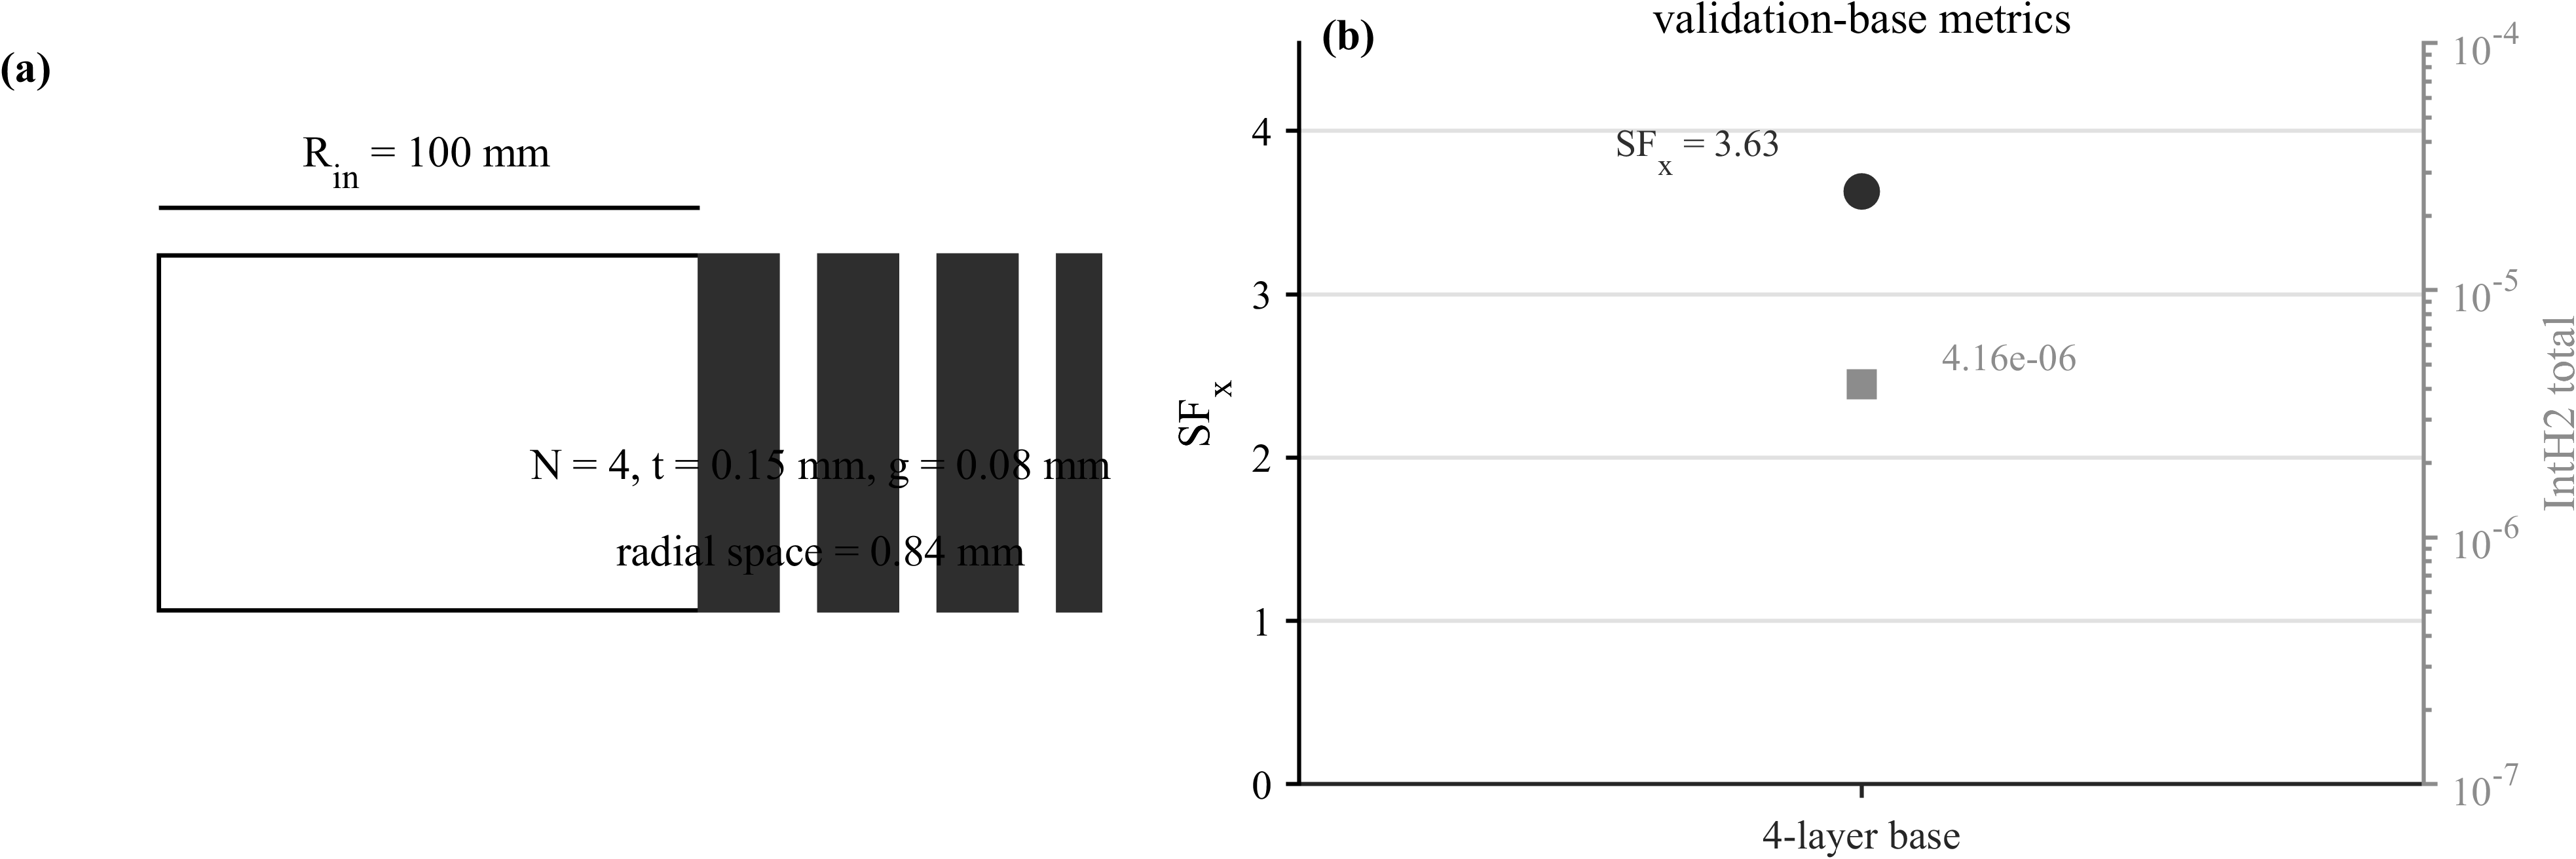
\includegraphics[width=\columnwidth]{Fig02_ferrite_base_selection.png}
\caption{Four-layer ferrite validation base. (a) Geometrical parameters of the selected manufacturable candidate. (b) Baseline shielding factor and IntH2 metric summary.}
\label{fig:ferritebase}
\end{figure}

\subsection{Simulation Matrix}

Table~\ref{tab:matrix} lists the simulation cases used for the revised paper claims. The P0 case is intentionally a screened reference rather than a no-shield reference, because a no-shield SERF residual field may be too large to measure in a practical setup.

\begin{table*}[!t]
\caption{Hybrid Ferrite Shield Simulation Matrix}
\label{tab:matrix}
\centering
\footnotesize
\setlength{\tabcolsep}{4pt}
\begin{tabular}{p{0.24\textwidth}p{0.12\textwidth}p{0.12\textwidth}p{0.12\textwidth}p{0.12\textwidth}p{0.22\textwidth}}
\toprule
Case & Base & Added material & Field dir. & Main output & Purpose \\
\midrule
$B0$ reference $x$ & no shield & none & $x$ & $B_{0,x}$ & transverse calibration \\
$B0$ reference $z$ & no shield & none & $z$ & $B_{0,z}$ & axial calibration \\
C2\_N4\_t015\_g008\_x & 4-layer ferrite & none & $x$ & $\mathrm{SF}_x$, IntH2 & manufacturable ferrite base \\
Hybrid AM outer layer & 4-layer ferrite & amorphous, \SI{0.20}{mm} & $x$ & $\mathrm{SF}_x$, $\mathrm{IntH2}_{\mathrm{outer}}$ & hybrid enhancement \\
Hybrid NC outer layer & 4-layer ferrite & nanocrystalline, \SI{0.20}{mm} & $x$ & $\mathrm{SF}_x$, $\mathrm{IntH2}_{\mathrm{outer}}$ & preferred simulated hybrid candidate \\
Open ferrite cylinder & 4-layer ferrite & none & $z$ & $\mathrm{SF}_z$, IntH2 & axial leakage baseline \\
P0 shell-cap & amorphous shell & amorphous single cap & $z$ & $\mathrm{SF}_z$, IntH2 & screened prototype reference \\
NC single cap & 4-layer ferrite & nanocrystalline cap & $z$ & $\mathrm{SF}_z$, IntH2 & axial cap tradeoff \\
\bottomrule
\end{tabular}
\end{table*}

\subsection{Geomagnetic Residual-Field Scaling}

The FEM excitation field is approximately \SI{1.2566}{\micro T}, not a nonlinear geomagnetic-field simulation. For engineering interpretation, the simulated $\mathrm{SF}$ values are scaled to a representative \SI{50}{\micro T} geomagnetic field:
\begin{equation}
B_{\mathrm{res,geo}}=\frac{\SI{50}{\micro T}}{\mathrm{SF}} .
\label{eq:geomagscale}
\end{equation}
This estimate is valid only under the linear initial-permeability assumption. It indicates residual-field order of magnitude and the need for compensation coils, but it does not replace nonlinear $B$--$H$ modeling or experimental nulling.

\section{Simulation Results and Structural Optimization}

\subsection{Four-Layer Ferrite Baseline}

For the transverse field direction, the four-layer ferrite-only base gives $\mathrm{SF}_x=3.629$ and $\mathrm{IntH2}_{\mathrm{total}}=4.160\times10^{-6}$. This confirms that the ferrite stack is a practical low-conductivity base, but its attenuation is limited when used alone. The design is therefore a base candidate for hybrid enhancement.

\subsection{Hybrid Outer-Layer Enhancement}

Compared with the ferrite-only base, the amorphous outer layer increases $\mathrm{SF}_x$ from 3.63 to 8.55, while the nanocrystalline outer layer further increases $\mathrm{SF}_x$ to 25.15. Meanwhile, $\mathrm{IntH2}_{\mathrm{total}}$ decreases from $4.16\times10^{-6}$ to $6.28\times10^{-7}$ and $5.33\times10^{-8}$ for the amorphous and nanocrystalline hybrid cases, respectively. The IntH2 integration includes both the ferrite layers and the added outer high-permeability layer.

\begin{figure}[!t]
\centering
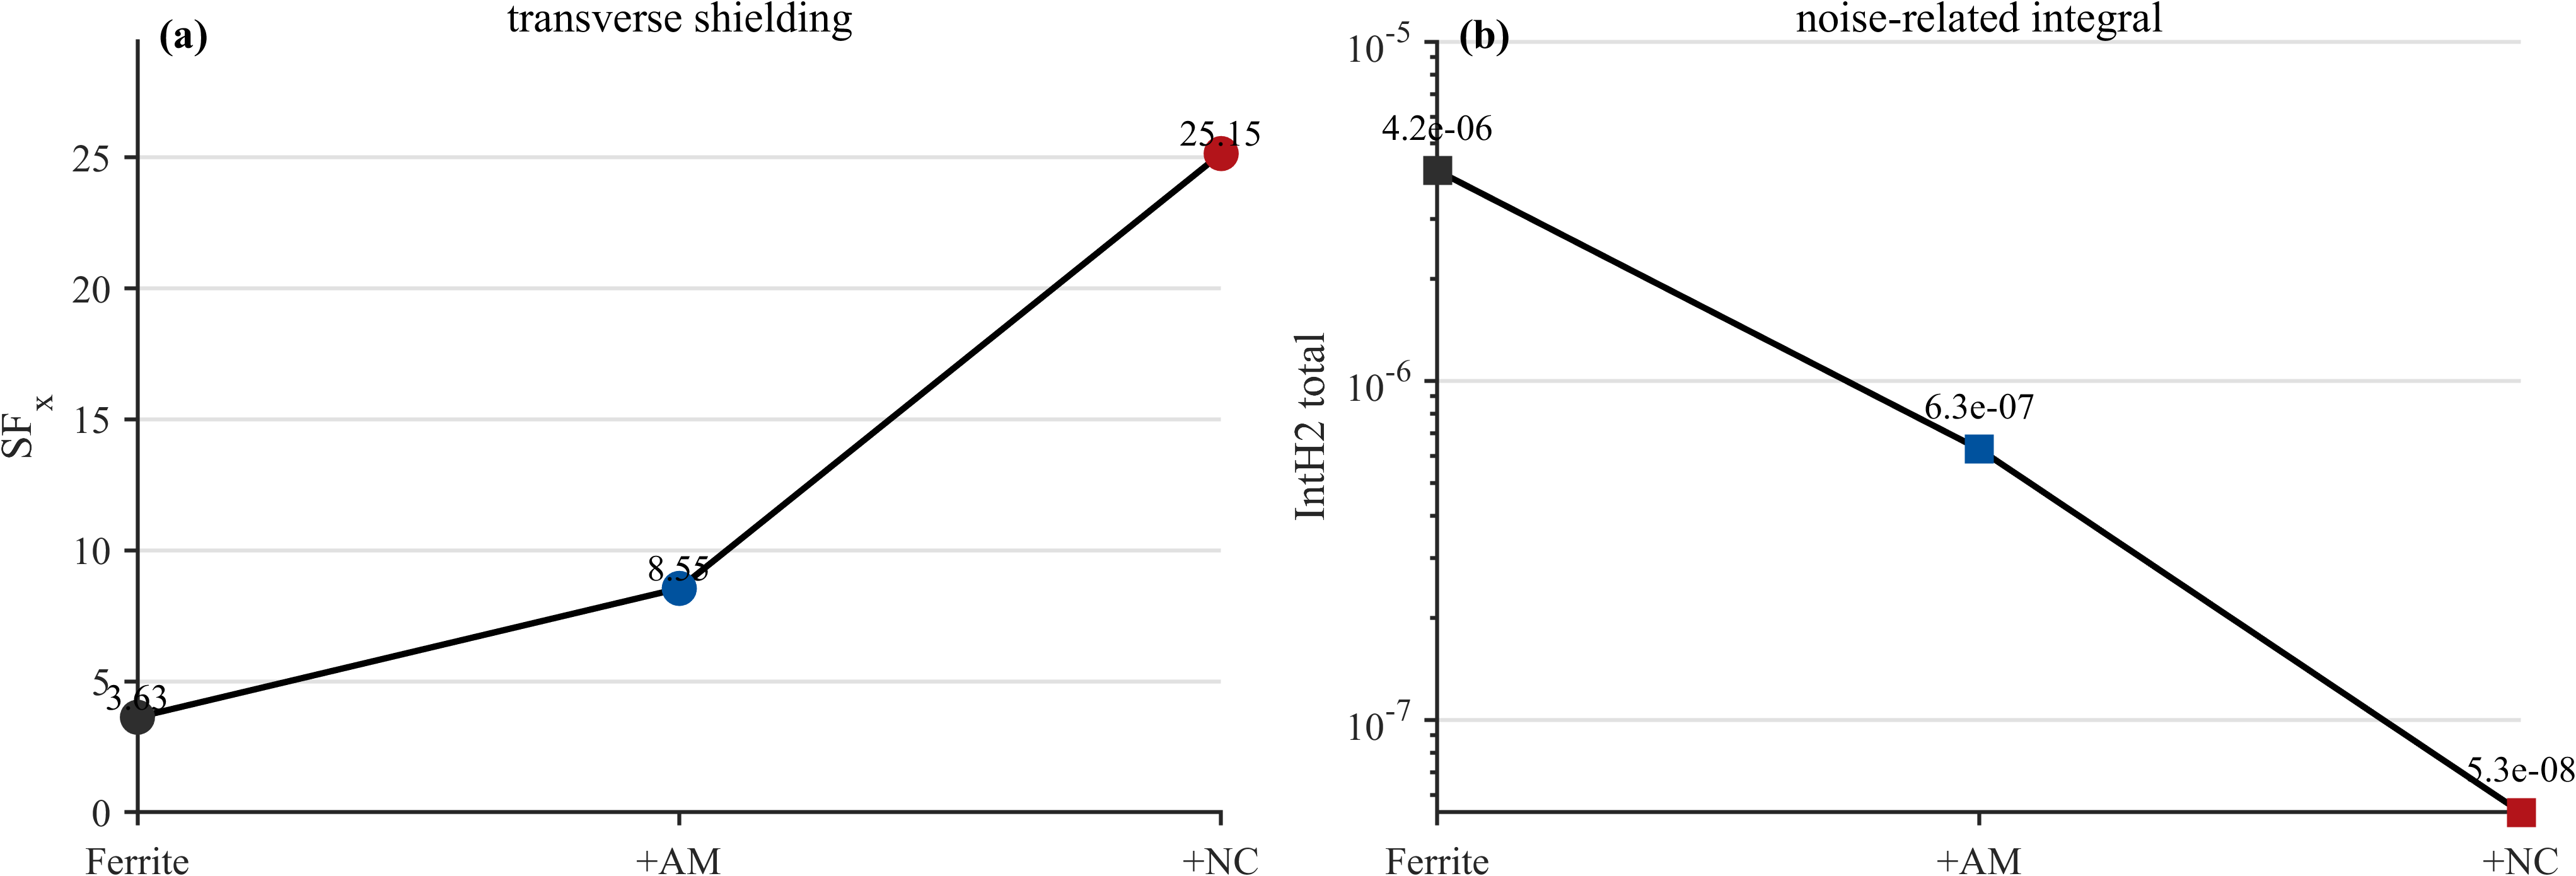
\includegraphics[width=\columnwidth]{Fig03_hybrid_outer_layer_enhancement.png}
\caption{Hybrid outer-layer enhancement in the transverse field direction. AM: amorphous; NC: nanocrystalline. (a) Shielding factor $\mathrm{SF}_x$. (b) Noise-related integral $\mathrm{IntH2}_{\mathrm{total}}$.}
\label{fig:hybrid}
\end{figure}

The nanocrystalline outer layer is selected as the current simulated priority candidate because it gives the highest $\mathrm{SF}_x$ and the lowest $\mathrm{IntH2}_{\mathrm{total}}$ among the present hybrid cases. This is a simulation-stage preference, not a measured magnetic-noise conclusion.

\subsection{Axial Single-Cap Tradeoff}

The open four-layer ferrite cylinder gives $\mathrm{SF}_z=2.412$ and $\mathrm{LeakageRatio}_z\approx0.4145$. The P0 amorphous shell-cap reference gives $\mathrm{SF}_z=2.526$ and $\mathrm{IntH2}_{\mathrm{total}}=3.960\times10^{-7}$. The four-layer ferrite shield with a single nanocrystalline cap improves $\mathrm{SF}_z$ to 2.907 and reduces the leakage ratio to 0.3440, but $\mathrm{IntH2}_{\mathrm{total}}$ increases relative to the open ferrite axial case. The cap is therefore an axial shielding improvement with a magnetic-noise-related tradeoff.

\begin{figure}[!t]
\centering
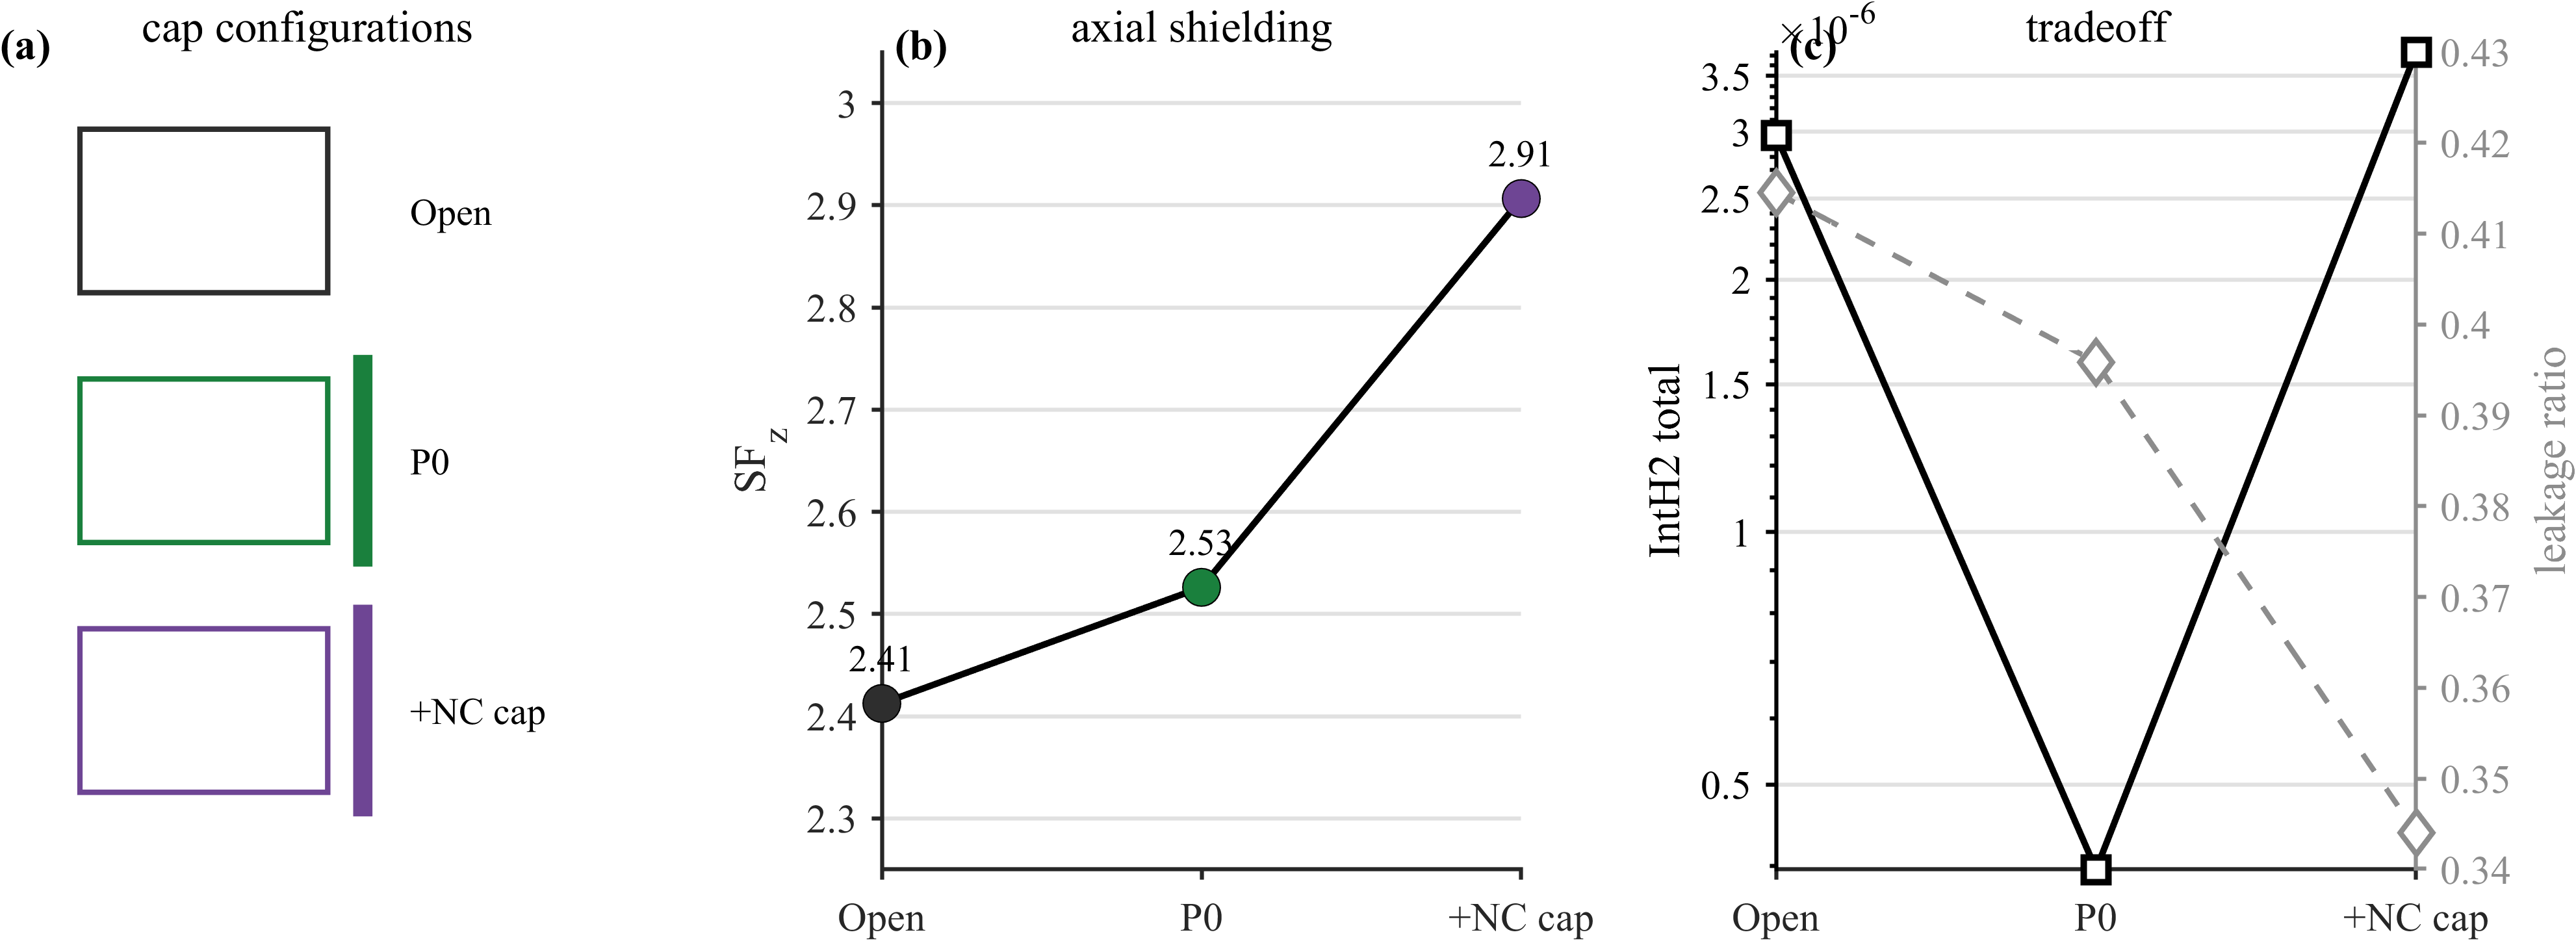
\includegraphics[width=\columnwidth]{Fig04_axial_cap_tradeoff.png}
\caption{Axial cap tradeoff. NC: nanocrystalline. (a) Axial shielding factor $\mathrm{SF}_z$. (b) $\mathrm{IntH2}_{\mathrm{total}}$. (c) Leakage ratio.}
\label{fig:axialcap}
\end{figure}

\subsection{Residual Field Under 50 $\mu$T Scaling}

Under linear scaling to a \SI{50}{\micro T} external field, the estimated transverse residual field decreases from \SI{13.78}{\micro T} for the ferrite-only base to \SI{5.85}{\micro T} with the amorphous outer layer and \SI{1.99}{\micro T} with the nanocrystalline outer layer. In the axial direction, the open ferrite case gives approximately \SI{20.73}{\micro T}, the P0 amorphous shell-cap reference gives approximately \SI{19.79}{\micro T}, and the nanocrystalline single-cap case gives approximately \SI{17.20}{\micro T}. These residual fields remain at the microtesla level, so compensation-coil nulling is required before SERF magnetometer PSD measurement.

\begin{figure}[!t]
\centering
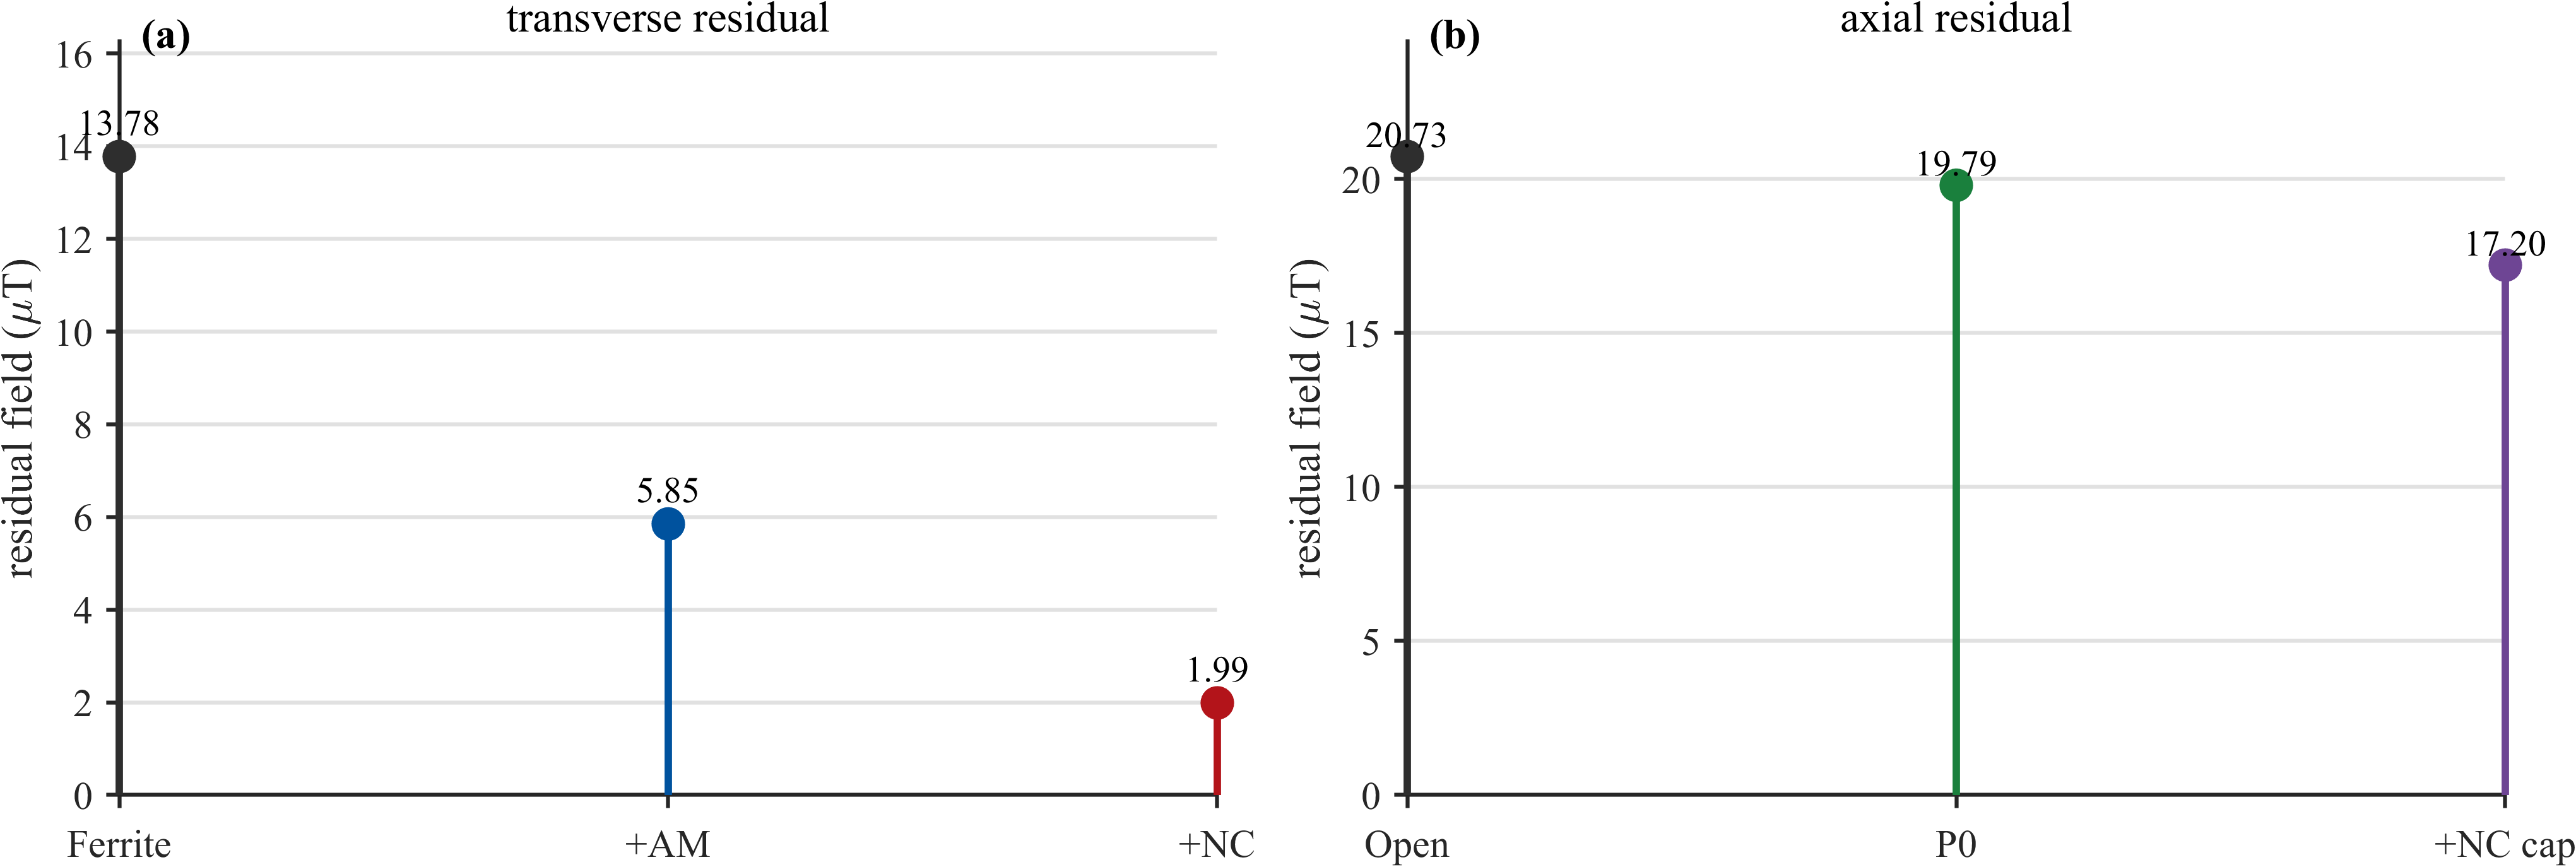
\includegraphics[width=\columnwidth]{Fig05_geomagnetic_residual_estimate.png}
\caption{Estimated residual field under a \SI{50}{\micro T} geomagnetic field using linear SF scaling. AM: amorphous; NC: nanocrystalline. (a) Transverse field. (b) Axial field.}
\label{fig:geomag}
\end{figure}

\subsection{Material-Loss Sensitivity}

The hybrid conclusion depends on both geometry and material loss. A sensitivity sweep of $\mu''_{\mathrm{metal}}/\mu''_{\mathrm{ferrite}}$ defines the risk that the non-ferrite ribbon has larger magnetic loss than the ferrite base. The nanocrystalline case remains attractive geometrically, but measured amorphous and nanocrystalline $\mu''(f)$ values are required before converting the IntH2 trend into a noise claim.

\begin{figure}[!t]
\centering
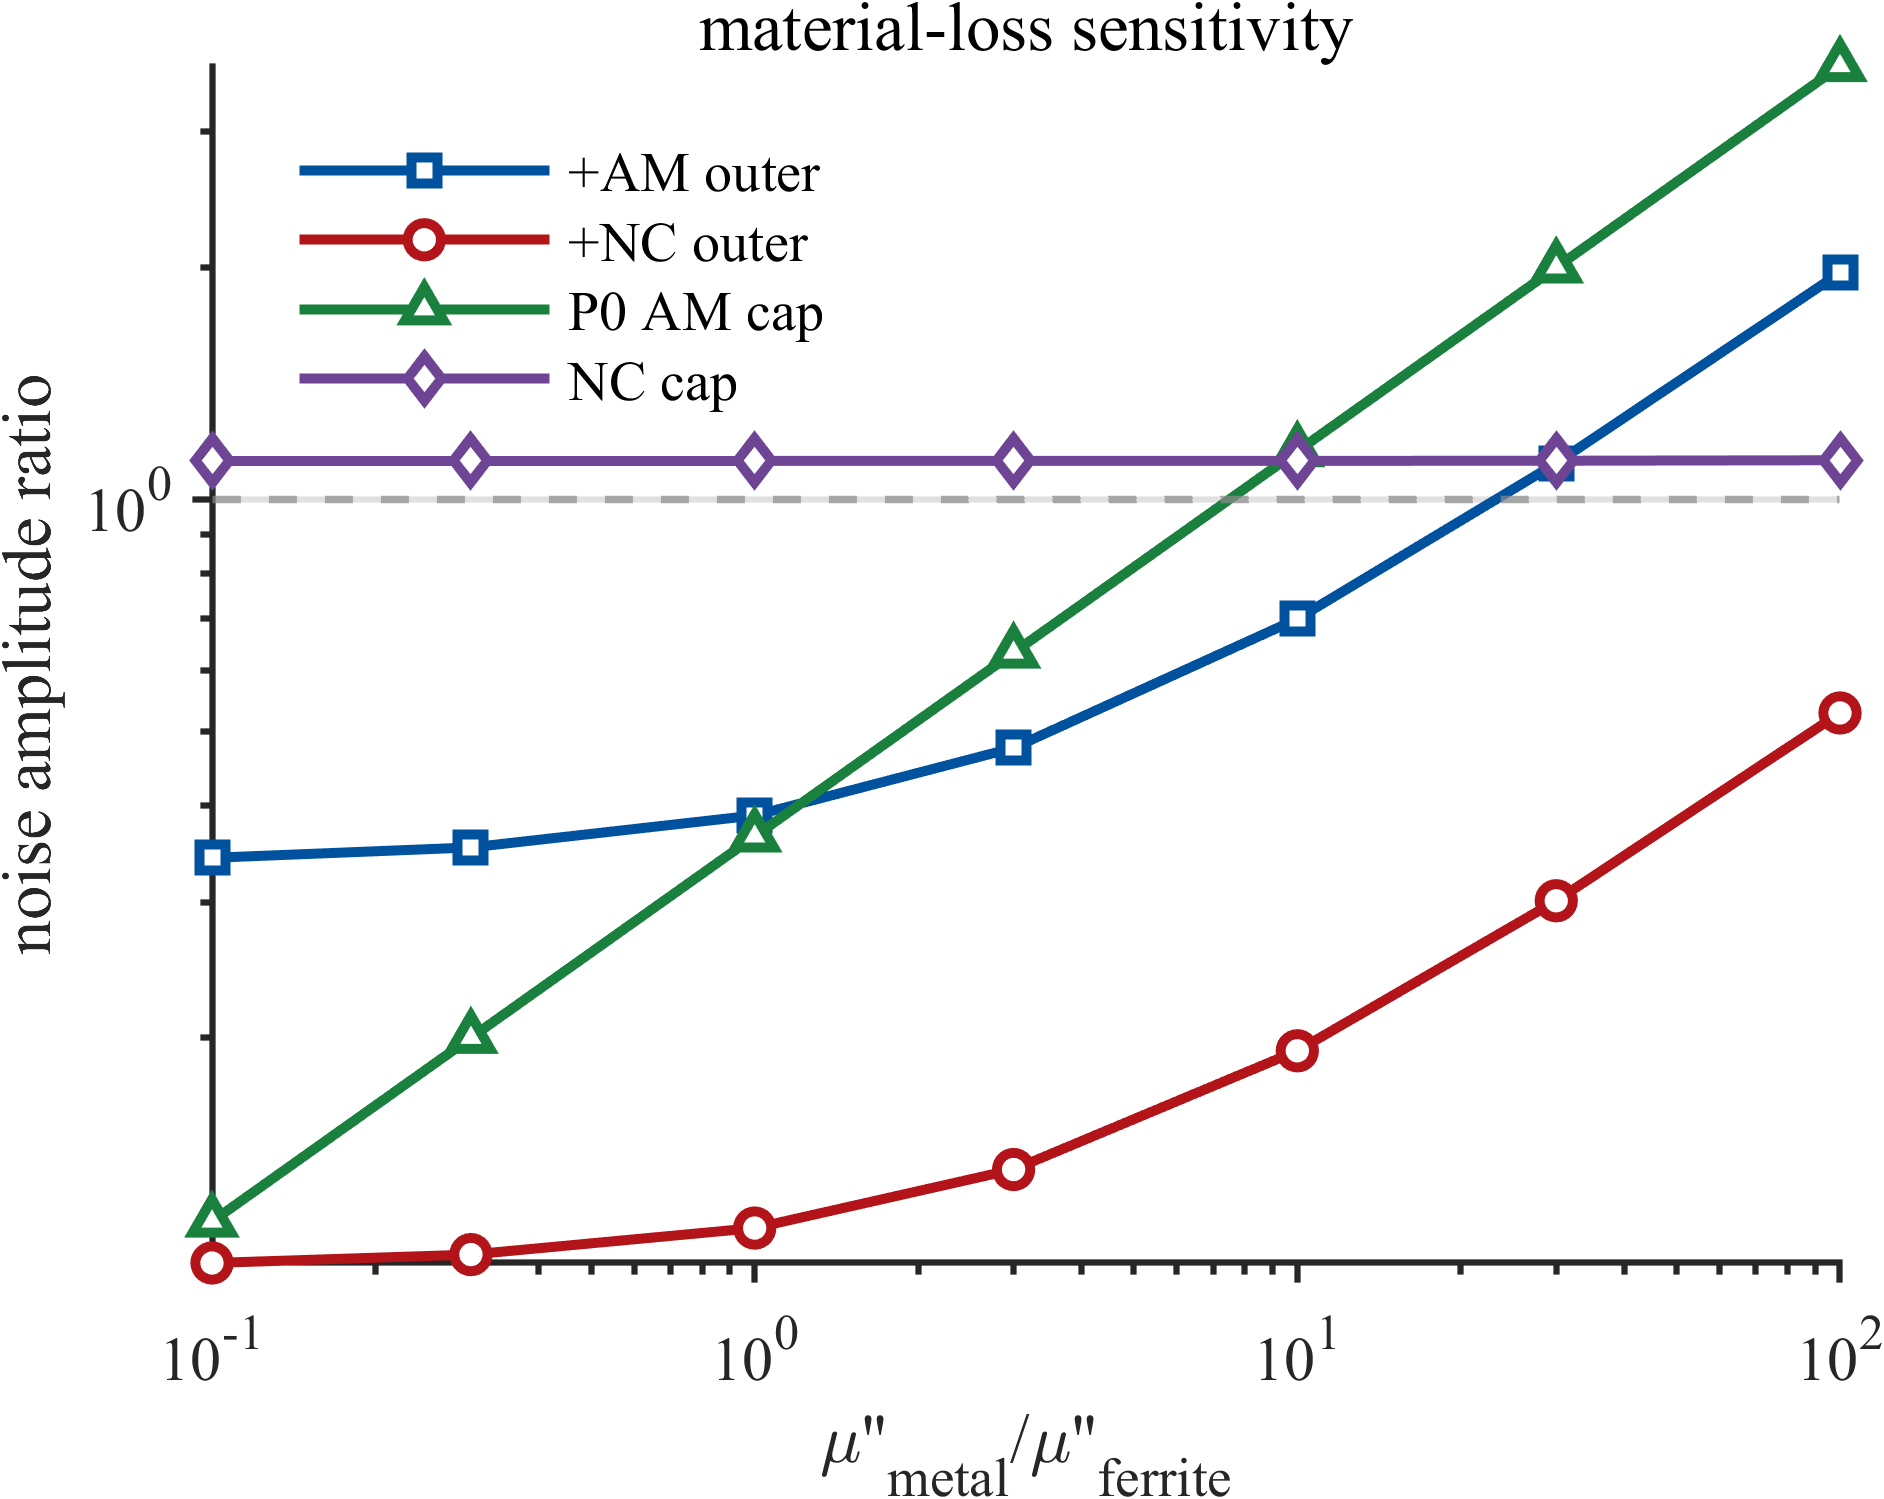
\includegraphics[width=\columnwidth]{Fig06_material_loss_sensitivity.png}
\caption{Sensitivity of the noise-amplitude proxy to the assumed magnetic loss of amorphous or nanocrystalline materials.}
\label{fig:loss}
\end{figure}

\section{Discussion and Experimental Validation Route}

\subsection{Prototype Shielding-Factor Measurement}

The prototype route is organized around three configurations: P0, a single amorphous shell plus a single $+z$ amorphous cap; P1, a four-layer ferrite prototype; and P2, a four-layer ferrite prototype with the selected nanocrystalline outer layer. Optional two-layer ferrite samples can be added to document bending and assembly limits. At minimum, the prototype comparison should report $x$- and $z$-directed shielding factors for P0, P1, and P2.

\subsection{Compensation-Coil Nulling and PSD Measurement}

Because the residual-field estimate remains at the microtesla level under \SI{50}{\micro T} scaling, a SERF or OPM experiment must include three-axis compensation-coil nulling. The relevant system quantities include residual DC field, peak-to-peak drift, and magnetometer PSD. Only after the P0/P1/P2 shielding factors, material permeability/loss measurements, compensation-coil nulling, and PSD data are available should the paper claim final sensitivity improvement.

\subsection{Application-Oriented Interpretation}

The long-term application target is a lightweight and potentially wearable magnetic shielding route for OPM- or SERF-based biomagnetic measurements. The present work supports this direction through modeling and prototype planning, but it does not claim that wearable MEG or final SERF sensitivity has already been realized.

\section{Conclusion}

A hybrid multilayer ferrite magnetic shield has been formulated for SERF-MEG magnetometer applications. The four-layer ferrite base is selected as a manufacturable validation candidate under thickness, flexibility, assembly, $\mathrm{SF}$, and IntH2 constraints, not as a global optimum. In transverse simulations, the ferrite-only base gives $\mathrm{SF}_x=3.629$ and $\mathrm{IntH2}_{\mathrm{total}}=4.160\times10^{-6}$. Adding an amorphous outer layer increases $\mathrm{SF}_x$ to 8.548, while adding a nanocrystalline outer layer increases $\mathrm{SF}_x$ to 25.146 and reduces $\mathrm{IntH2}_{\mathrm{total}}$ to $5.333\times10^{-8}$ under the present initial-permeability assumptions. Axial cap simulations show that a single nanocrystalline cap improves $\mathrm{SF}_z$ but introduces an IntH2 tradeoff. The current conclusions remain conditional: amorphous and nanocrystalline permeability values represent low-field initial-permeability assumptions, material loss must be measured, and prototype SF and PSD tests are required before claiming instrument-level sensitivity improvement.

\section*{Acknowledgment}
Funding, facilities, and collaborator acknowledgments should be added before submission.

\begin{thebibliography}{31}

\bibitem{ref1}
J.~C.~Allred, R.~N.~Lyman, T.~W.~Kornack, and M.~V.~Romalis,
``High-sensitivity atomic magnetometer unaffected by spin-exchange relaxation,''
\textit{Phys. Rev. Lett.}, vol.~89, no.~13, Sep.~2002, Art.~no.~130801.

\bibitem{ref2}
I.~K.~Kominis, T.~W.~Kornack, J.~C.~Allred, and M.~V.~Romalis,
``A subfemtotesla multichannel atomic magnetometer,''
\textit{Nature}, vol.~422, no.~6932, pp.~596--599, Apr.~2003.

\bibitem{ref3}
M.~P.~Ledbetter, I.~M.~Savukov, V.~Acosta, D.~Budker, and M.~V.~Romalis,
``Spin-exchange-relaxation-free magnetometry with Cs vapor,''
\textit{Phys. Rev. A}, vol.~77, no.~3, Mar.~2008, Art.~no.~033408.

\bibitem{ref4}
S.~Baillet,
``Magnetoencephalography for brain electrophysiology and imaging,''
\textit{Nature Neurosci.}, vol.~20, no.~3, pp.~327--339, Mar.~2017.

\bibitem{ref6}
T.~J.~Sumner, J.~M.~Pendlebury, and K.~F.~Smith,
``Conventional magnetic shielding,''
\textit{J. Phys. D: Appl. Phys.}, vol.~20, no.~9, pp.~1095--1101, Sep.~1987.

\bibitem{ref7}
V.~Kelha, J.~Pukki, R.~Peltonen, A.~Penttinen, R.~Ilmoniemi, and J.~Heino,
``Design, construction, and performance of a large-volume magnetic shield,''
\textit{IEEE Trans. Magn.}, vol.~18, no.~1, pp.~260--270, Jan.~1982.

\bibitem{ref8}
I.~Altarev \textit{et al.},
``A magnetically shielded room with ultra low residual field and gradient,''
\textit{Rev. Sci. Instrum.}, vol.~85, no.~7, Jul.~2014, Art.~no.~075106.

\bibitem{ref9}
S.-K.~Lee and M.~V.~Romalis,
``Calculation of magnetic field noise from high-permeability magnetic shields and conducting objects with simple geometry,''
\textit{J. Appl. Phys.}, vol.~103, no.~8, Apr.~2008, Art.~no.~084904.

\bibitem{ref10}
H.~B.~Dang, A.~C.~Maloof, and M.~V.~Romalis,
``Ultrahigh sensitivity magnetic field and magnetization measurements with an atomic magnetometer,''
\textit{Appl. Phys. Lett.}, vol.~97, no.~15, Oct.~2010, Art.~no.~151110.

\bibitem{ref11}
D.~Ma \textit{et al.},
``A novel low-noise mu-metal magnetic shield with winding shape,''
\textit{Sens. Actuators A, Phys.}, vol.~346, Oct.~2022, Art.~no.~113884.

\bibitem{ref12}
T.~W.~Kornack, S.~J.~Smullin, S.-K.~Lee, and M.~V.~Romalis,
``A low-noise ferrite magnetic shield,''
\textit{Appl. Phys. Lett.}, vol.~90, no.~22, May~2007, Art.~no.~223501.

\bibitem{ref13}
D.~Ma \textit{et al.},
``Parameter modeling analysis of a cylindrical ferrite magnetic shield to reduce magnetic noise,''
\textit{IEEE Trans. Ind. Electron.}, vol.~69, no.~1, pp.~991--998, Jan.~2022.

\bibitem{ref14}
J.~Lu \textit{et al.},
``Study of magnetic noise of a multi-annular ferrite shield,''
\textit{IEEE Access}, vol.~8, pp.~40918--40924, 2020.

\bibitem{ref16}
B.~Sun \textit{et al.},
``Suppression of magnetic noise and field in cubic low-noise ferrite magnetic shields,''
\textit{IEEE Trans. Instrum. Meas.}, vol.~73, pp.~1--10, 2024, Art.~no.~1501810.

\bibitem{ref18}
R.~Kubo,
``The fluctuation-dissipation theorem,''
\textit{Rep. Prog. Phys.}, vol.~29, no.~1, pp.~255--284, Jan.~1966.

\bibitem{ref30}
J.~Fang, S.~Wan, J.~Qin, and Y.~Chen,
``A novel method for in-situ measuring the static shielding factor of a magnetic shield,''
\textit{Measurement}, vol.~170, 2021, Art.~no.~108718.

\bibitem{ref31}
T.~Brys \textit{et al.},
``Magnetic field stabilization for magnetically shielded volumes by external field coils,''
\textit{J. Appl. Phys.}, vol.~116, no.~8, 2014, Art.~no.~084903.

\end{thebibliography}

\end{document}
